\documentclass{beamer}
\usepackage[utf8]{inputenc}
\usetheme{Copenhagen}
\usecolortheme{beaver}
\usepackage{graphicx}

\usepackage{bm}
\usepackage{listings,verbatim}
\usepackage{fancyvrb,tikz,color,xcolor,colortbl}

\newcommand{\p}{\pause}
\definecolor{Grey}{rgb}{0.95,0.95,0.95}
\newcommand{\pitem}{\pause \item}
\newenvironment{graytext}{\color{gray}}{\ignorespacesafterend}

\newcommand\independent{\protect\mathpalette{\protect\independenT}{\perp}}
\def\independenT#1#2{\mathrel{\rlap{$#1#2$}\mkern2mu{#1#2}}}

\definecolor{umassblue}{RGB}{51,51,153}
\definecolor{umassgreen}{RGB}{0,102,102}
%\definecolor{blue}{RGB}{51,51,153}
\definecolor{bblue}{RGB}{0,0,255}
\definecolor{red}{RGB}{153,0,51}

\newcommand\verbbf[1]{\textcolor[RGB]{51,51,153}{\textbf{$\blacksquare$ #1}}}
\newcommand\verbrf[1]{\textcolor[RGB]{153,0,51}{\textbf{$\blacksquare$ #1}}}

\newcommand{\N}{\mathcal{N}}
\newcommand{\Y}{\bm{\mathcal{Y}}}

\usefonttheme{serif}

\newenvironment{changemargin}[2]{%
	\begin{list}{}{%
			\setlength{\topsep}{0pt}%
			\setlength{\leftmargin}{#1}%
			\setlength{\rightmargin}{#2}%
			\setlength{\listparindent}{\parindent}%
			\setlength{\itemindent}{\parindent}%
			\setlength{\parsep}{\parskip}%
		}%
		\item[]}{\end{list}}


%\setbeamersize{text margin left=2pt,text margin right=2pt} 
\newcommand\Wider[2][3em]{%
	\makebox[\linewidth][c]{%
		\begin{minipage}{\dimexpr\textwidth+#1\relax}
			\raggedright#2
		\end{minipage}%
	}%
}

\newcommand\Wide[2][1.5em]{%
	\makebox[\linewidth][c]{%
		\begin{minipage}{\dimexpr\textwidth+#1\relax}
			\raggedright#2
		\end{minipage}%
	}%
}

\makeatletter
\setbeamertemplate{footline}
{
	\leavevmode%
	\hbox{%
		\begin{beamercolorbox}[wd=0.75\paperwidth,ht=2.25ex,dp=1ex,left]{title in head/foot}%
			\usebeamerfont{title in head/foot}\insertshorttitle{}
		\end{beamercolorbox}%
		\begin{beamercolorbox}[wd=0.25\paperwidth,ht=2.25ex,dp=1ex,right]{date in head/foot}%
			\insertframenumber{} / \inserttotalframenumber\hspace*{2ex} 
		\end{beamercolorbox}}%
		\vskip0pt%
	}
	\makeatother
	
	
	%Information to be included in the title page:
	\title[Hierartical Structure in Social Networks]{Hierartical Structure in Social Networks}
	\author{Cindy Cook, Matt Denny, Mitch Goist, Timmy Huynh}
	\institute{SODA502:  Final Project}
	\date{9 December 2015}
	
	
	\begin{document}
		
		\frame{\titlepage}
\begin{frame}\frametitle{Theorizing Hierarchy in Networks - Prior Work}
	\begin{changemargin}{-2cm}{ -2cm}
		\centering
		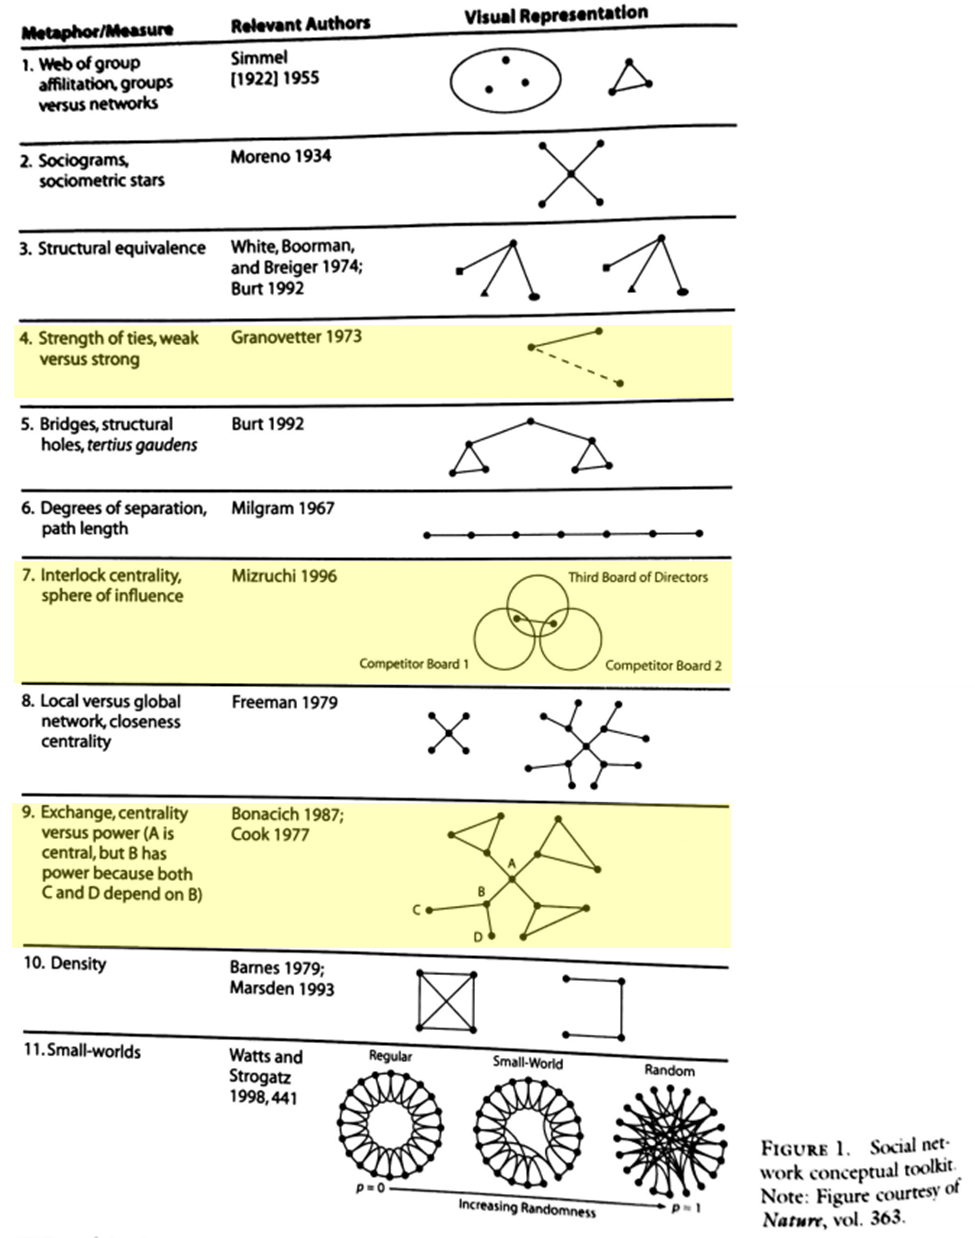
\includegraphics[width=8cm, height=8cm]{images/table_overview.png} 
	\end{changemargin}
\end{frame}

\begin{frame}\frametitle{Theorizing Hierarchy in Networks - Mann}
	\begin{changemargin}{-2cm}{ -2cm}
		\centering
		\hspace{-5cm}
		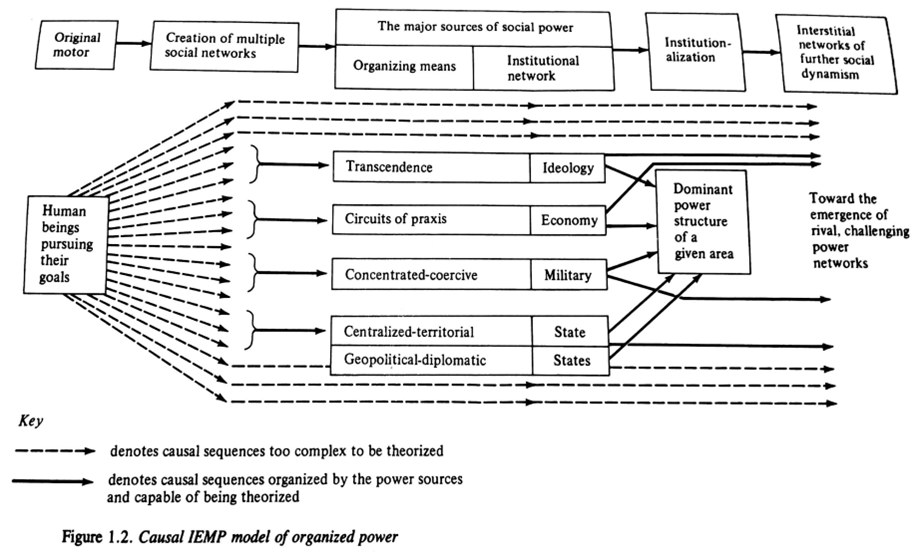
\includegraphics[width=7cm, height=5cm]{images/mann_overview.png} \\
		\hspace{5cm} 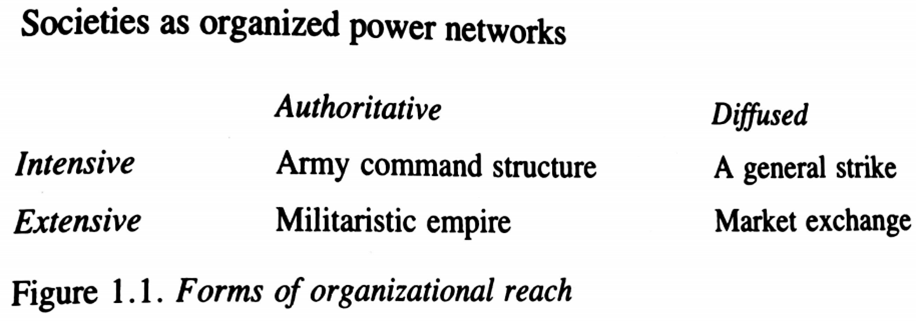
\includegraphics[width=8cm, height=3cm]{images/mann_typologies.png}
	\end{changemargin}
\end{frame}

\begin{frame}\frametitle{Hierarchy in networks--Measures}
	\begin{table}
		\begin{tabular}{| r || c | c | c | c |}
			\hline
			Measure & Undirected & Weighted & Global & Local \\
			\hline
			Landau's h & & X& X& \\
			Kendall's K & X& X& &X\\
			Reach Degree & X& X& &X\\
			Reach Closeness & X& X& &X\\
			GRC & X& X& X&X\\
			Rooted Depth & & & X&\\
			Degree & X& X& X&X\\
			Closeness & X& X& X&X\\
			Betweenness & X& X& X&X\\
			Eigenvector &  X& X& X& X \\
			\hline
		\end{tabular}
	\end{table}
\end{frame}

\begin{frame}\frametitle{Hierarchy in Networks--Simulated Datasets}
	\begin{itemize}
		\small{
		\item 7500 Barabasi-Albert (BA) Datasets with node size $50, 200,$ or $500$ and preferential attachment parameter $0.5, 1, 2, 5,$ or $10$.
		\item 6000 Tree-Structured (TR) Datasets with node size $50, 200,$ or $500$ and children parameter $2, 5, 10,$ or $50$.
		\item 4500 Erdos-Renyi (ER) Datasets with node size $50, 200,$ or $500$ and parameter size $0.05, 0.1,$ or $0.2$.}
		\scriptsize
			\begin{table}
				\begin{tabular}{| r || c | c | c |}
					\hline
					 BA and TR & Node & Edge & Density     \\
					\hline
					 &  50&  49&  0.02    \\	
					 &  200& 199&  0.005    \\
					 &  500& 499&  0.002    \\
					\hline
					\end{tabular}
				\end{table}
				\begin{table}
					\begin{tabular}{| r || c | c | c |c| c|}
						\hline
						ER & Node & Parameter& Edge & Density&Cluster Coefficient \\
						\hline
						& 50& 0.05&122.524 & 0.050 &  0.0956  \\
						  & 50& 0.1&244.768 & 0.100 &  0.188   \\
						  & 50& 0.2&490.050 & 0.200 &  0.359   \\	
						  &200&0.05&1989.242 &0.050&    0.098\\
						  &200&0.1&3980.776& 0.100&     0.190\\
						  &200&0.2&7952.138& 0.120&     0.360\\
						  &500&0.05&12473.270& 0.050&    0.097\\
						  &500&0.1&24932.824& 0.100&       0.190\\
						  &500&0.2&49892.784& 0.200&  0.360	\\			
						\hline
					\end{tabular}
				\end{table}
	\end{itemize}
\end{frame}

\begin{frame}\frametitle{Average Global Hierarchy--BA Networks}
	\begin{changemargin}{-2cm}{ -2cm}
		\centering
		 \text{Parameters}\par
		 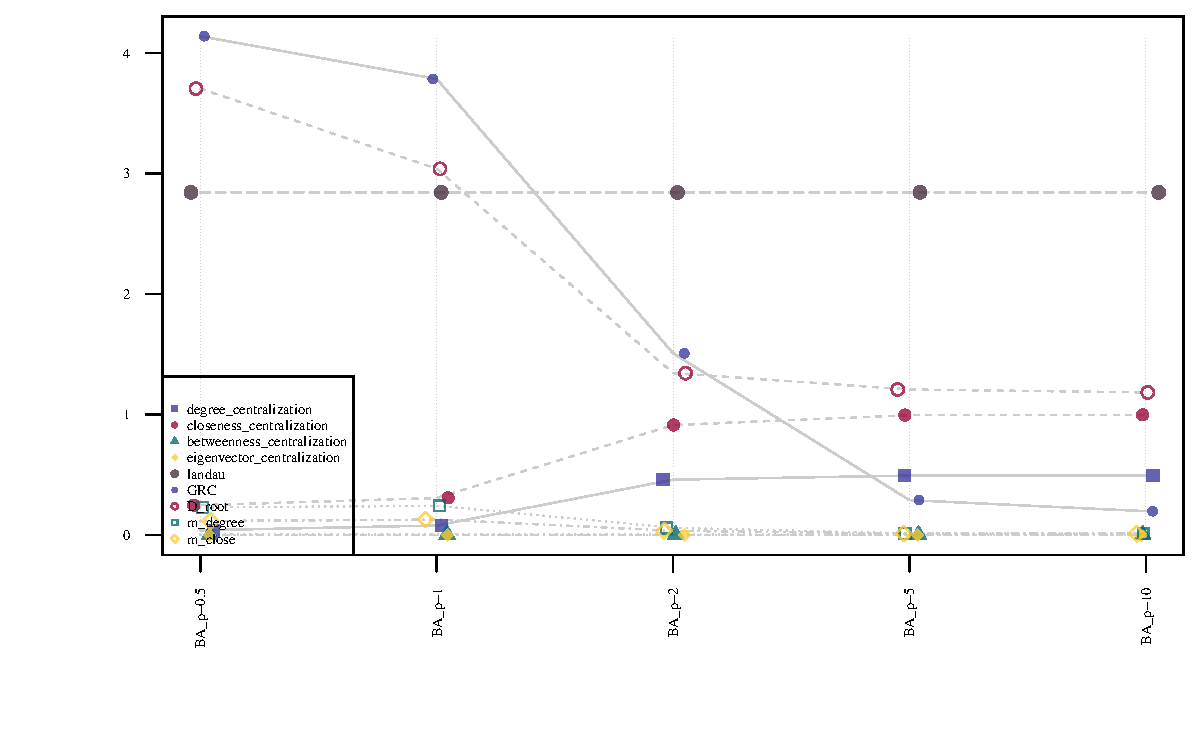
\includegraphics[width=10cm, height=4cm]{images/BA_Param_Averages.pdf}
		\\
		\vspace{-5mm}
		 \text{Node Size}\par
		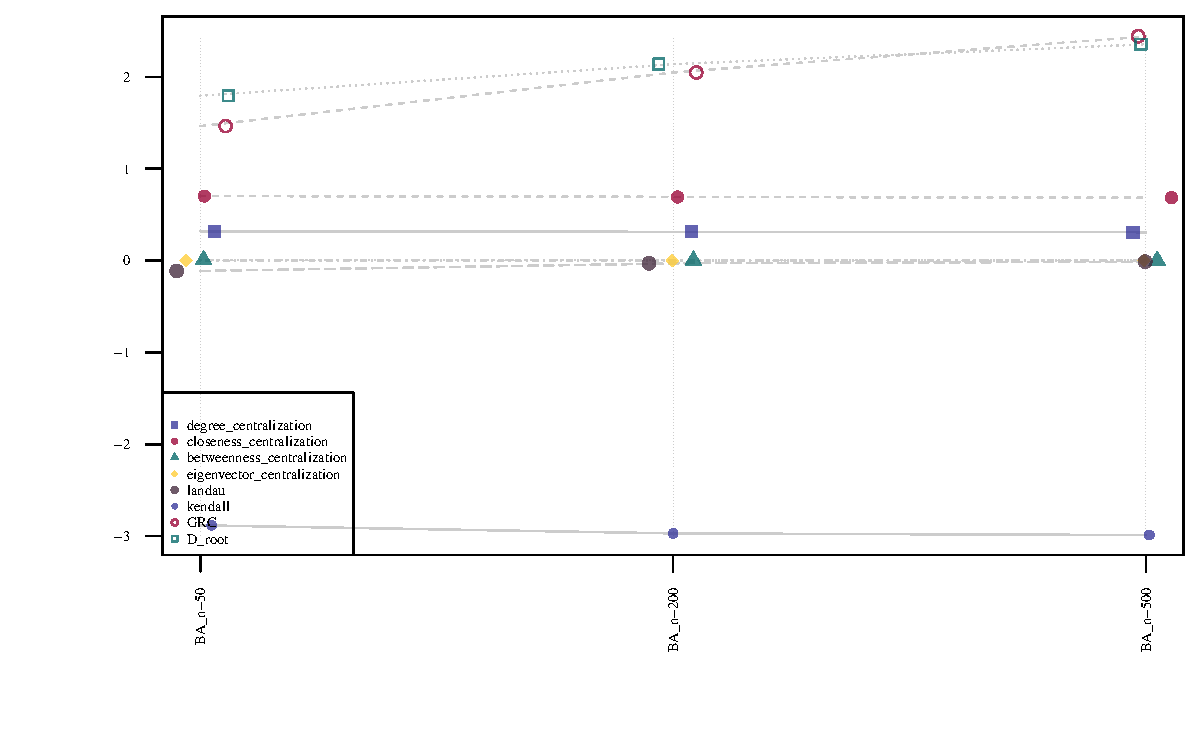
\includegraphics[width=10cm, height=4cm]{images/BA_Size_Averages.pdf}
	\end{changemargin}
\end{frame}


\begin{frame}\frametitle{Average Global Hierarchy--TR Networks}
	\begin{changemargin}{-2cm}{ -2cm}
		\centering
		\text{Parameters}\par
		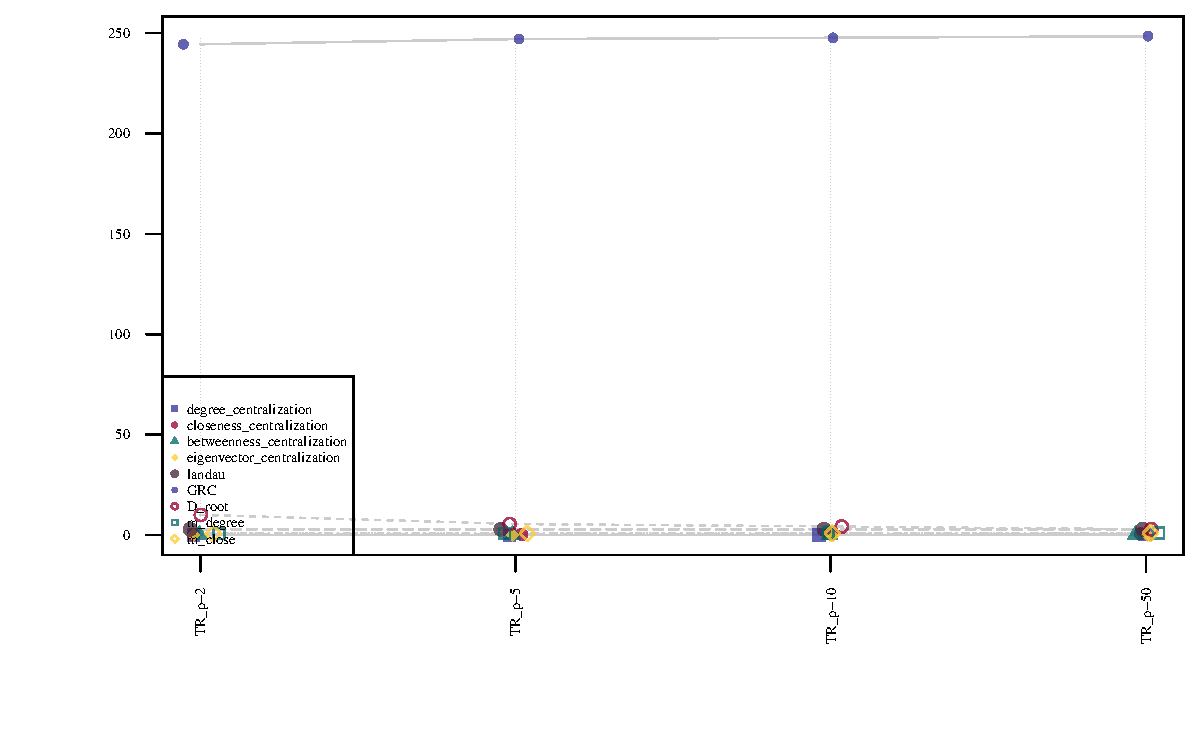
\includegraphics[width=10cm, height=4cm]{images/TR_Param_Averages.pdf}
		\\
		\vspace{-5mm}
		\text{Node Size}\par
		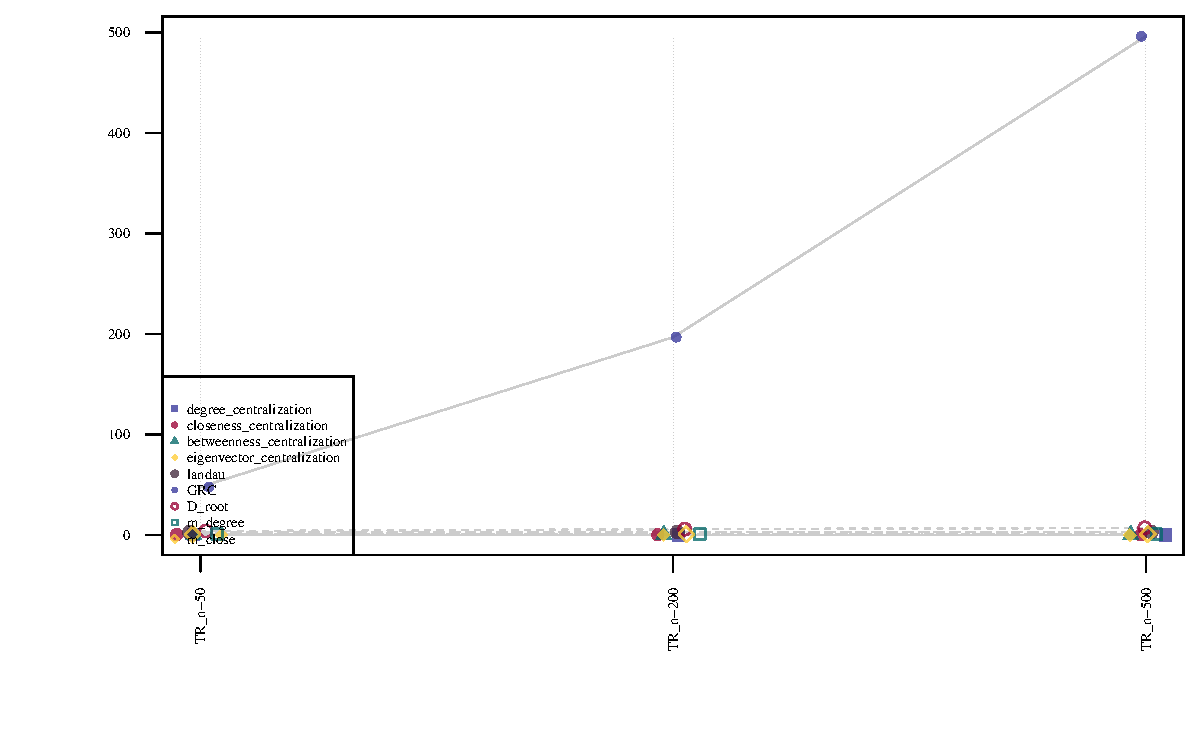
\includegraphics[width=10cm, height=4cm]{images/TR_Size_Averages.pdf}
	\end{changemargin}
\end{frame}

\begin{frame}\frametitle{Average Global Hierarchy--ER Networks}
	\begin{changemargin}{-2cm}{ -2cm}
		\centering
		\text{Parameters}\par
		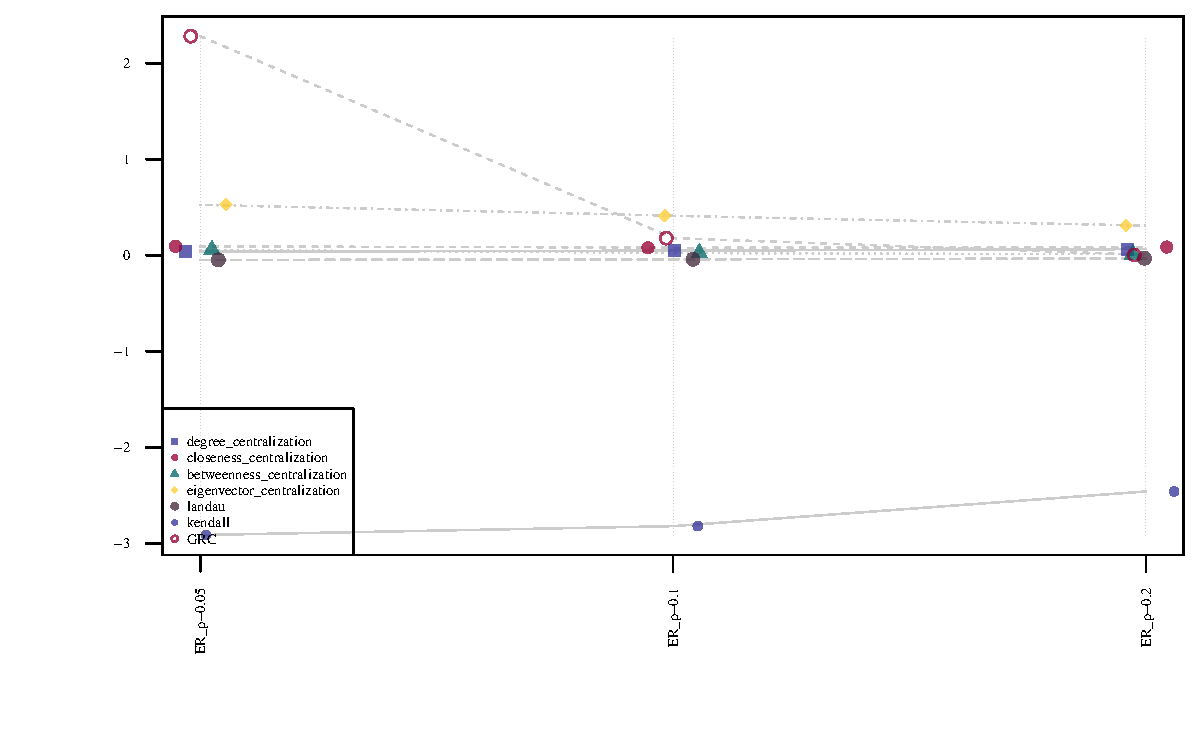
\includegraphics[width=10cm, height=4cm]{images/ER_Param_Averages.pdf}
		\\
		\vspace{-5mm}
		\text{Node Size}\par
		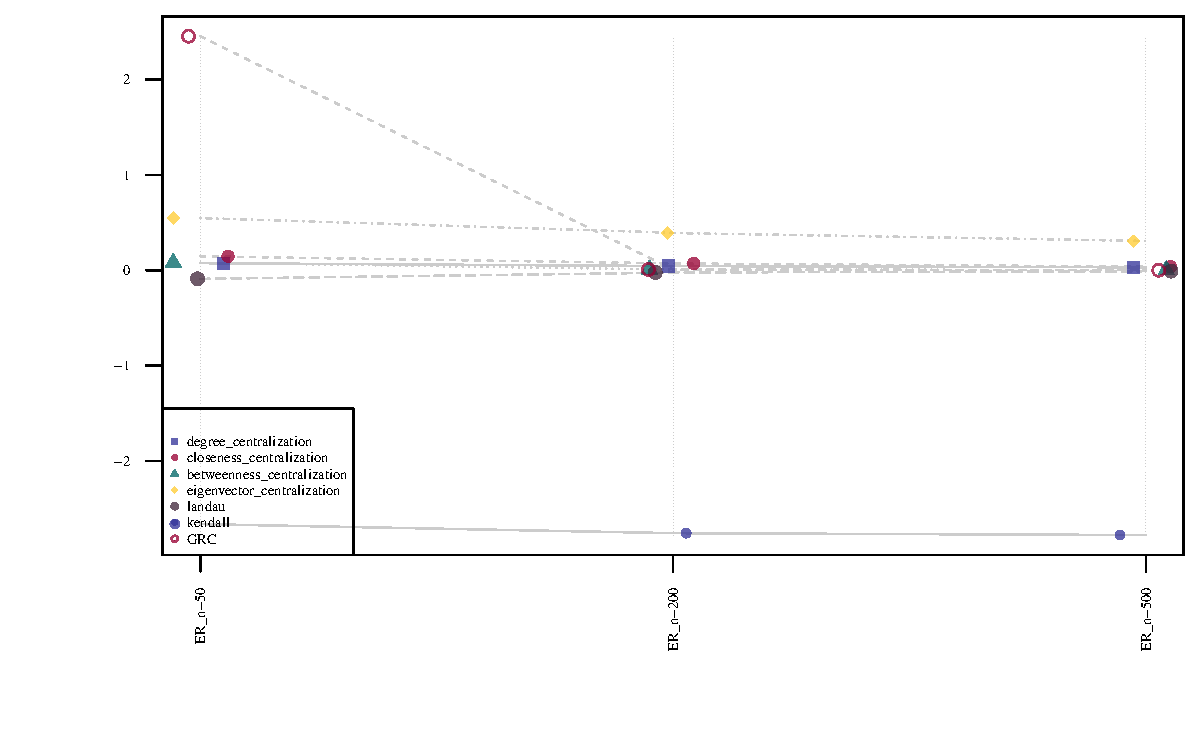
\includegraphics[width=10cm, height=4cm]{images/ER_Size_Averages.pdf}
	\end{changemargin}
\end{frame}

\begin{frame}\frametitle{Hierarchy in Networks--Results}
	\begin{itemize}
		\item GRC and D Root are not robust to changes in node size.
		\begin{itemize}
			\item GRC increases with node size for both BA and TR networks
			\item GRC decreases with node size for ER networks. 
			\item D Root increases with node size for BA networks.
		\end{itemize}
	\end{itemize}
\end{frame}

\begin{frame}\frametitle{Hierarchy in Networks--Datasets}
	\begin{itemize}
		\item 141 datasets from UCINET, organizational emails, and Congress
		\vspace{.2in}
		\scriptsize
		\begin{table}
			\begin{tabular}{| r || c | c | c | c |}
				\hline
				Type & Nodes & Edges & Density & Cluster Coeff. \\
				\hline
				Communication & 25.714  &2419  &3.483 &  0.558 \\
				Cosponsorship &101.222 &13358.889  &1.317  & 0.788\\
				Co-membership & 22  &9267.333 &18.318  & 0.377\\
				Interaction & 23.075 & 1944.95 & 1.985   &  0.589\\
				Unknown & 76.833 & 4688.25 & 0.360   &  	NaN\\
				Friendship & 29.833  &  92 & 0.122    &  0.348\\
				Affect & 17.636  &  95.182 & 0.319      &	0.329\\
				Terrorism & 63 &  308 & 0.079    &  0.361\\
				Trade & 24 &  285.6 & 0.5170     &  0.734\\
				\hline
			\end{tabular}
		\end{table}
	\end{itemize}
\end{frame}


\begin{frame}\frametitle{Hierarchy in Networks -- Global Measures}
\begin{changemargin}{-2cm}{ -2cm}
	\centering
	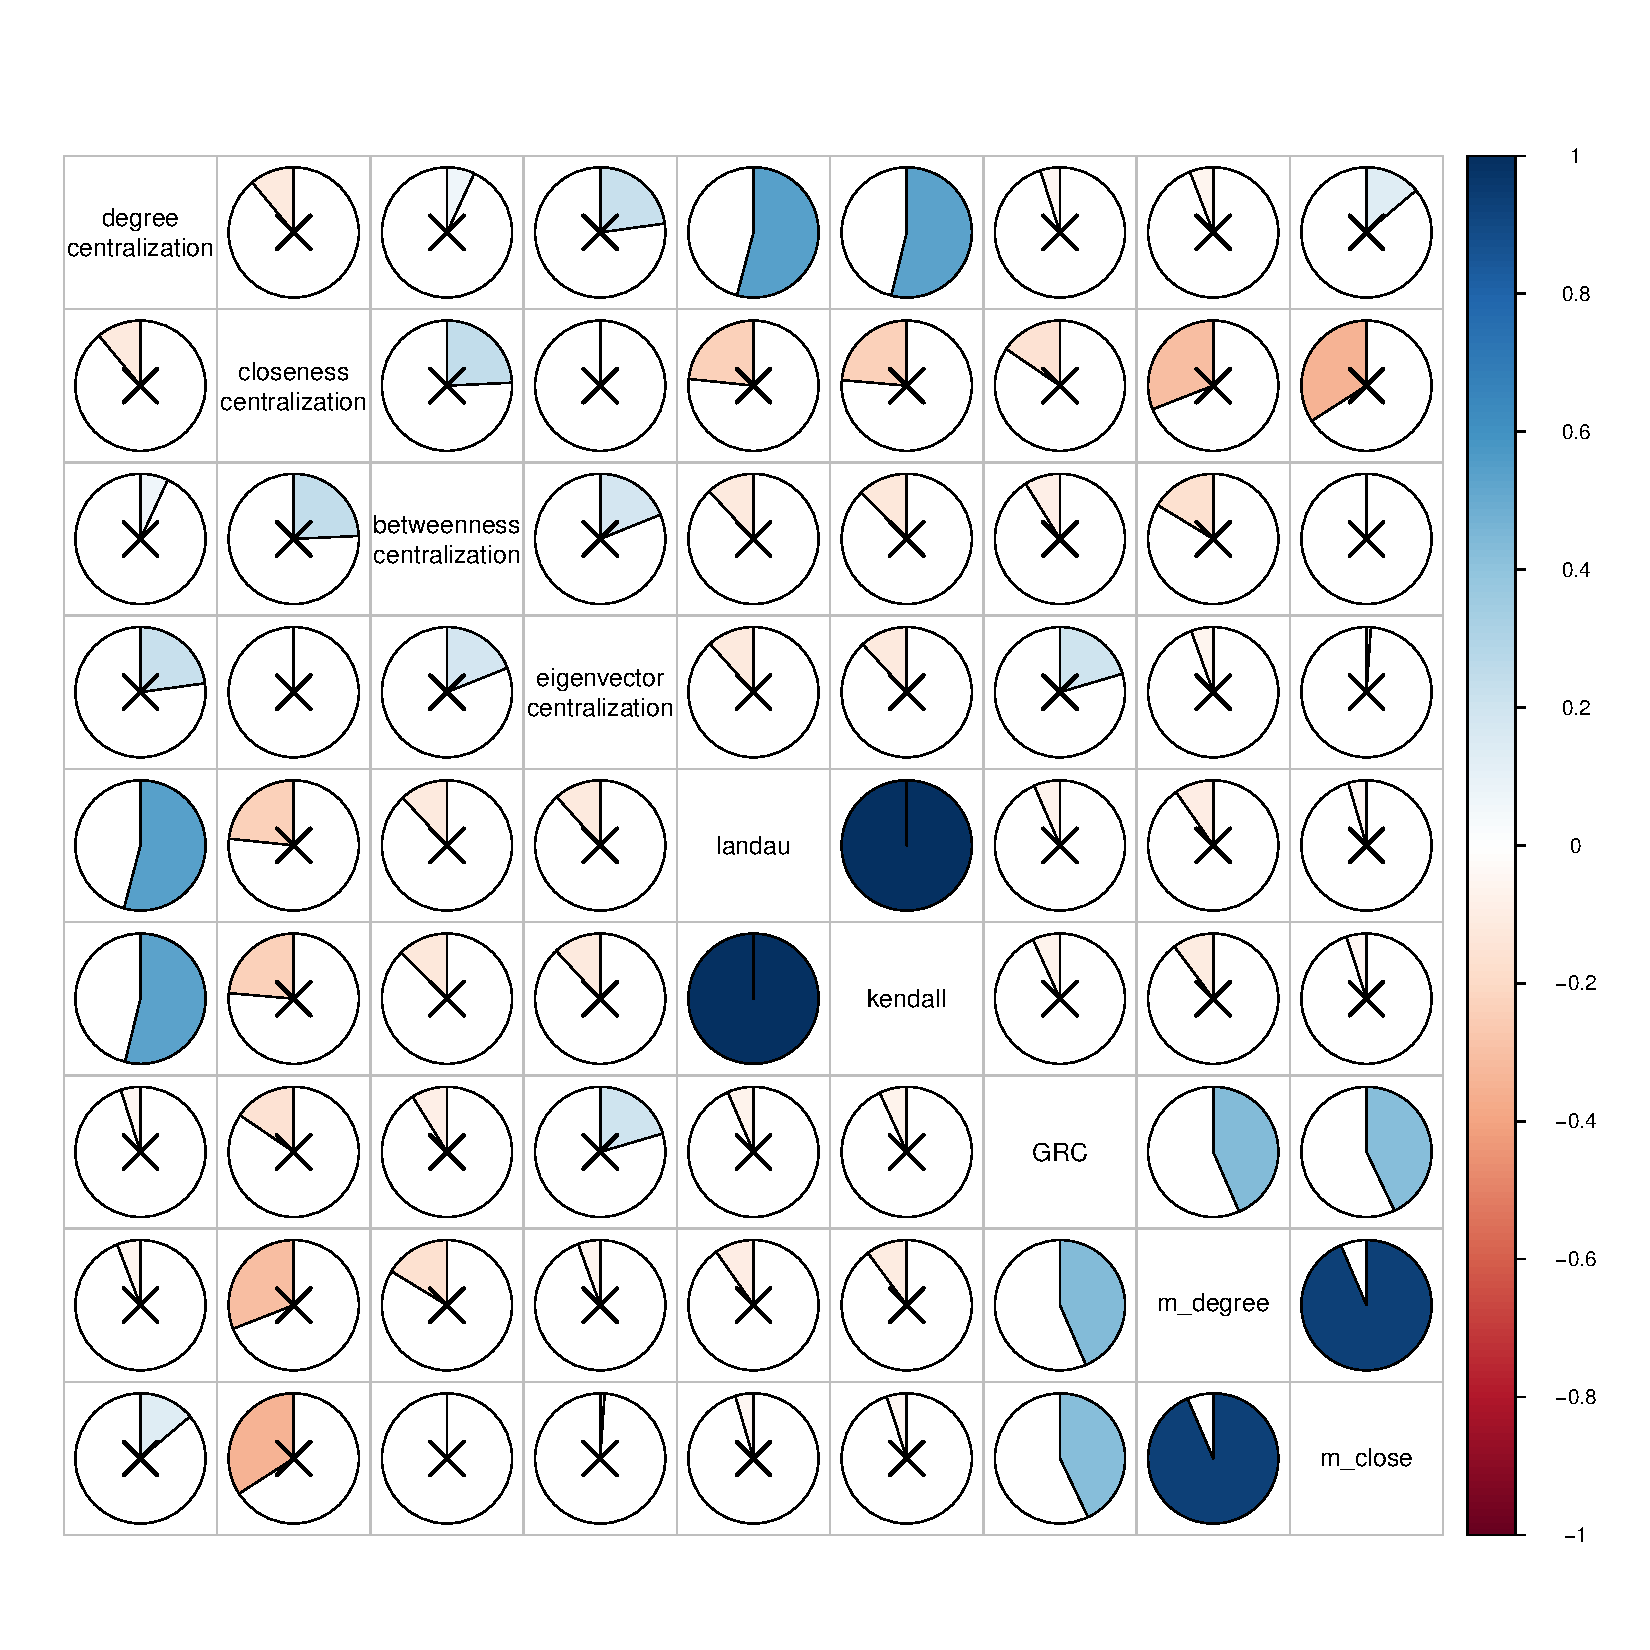
\includegraphics[width=12cm, height=8cm]{images/Global_Measure_Correlations_with_Tests.pdf}
\end{changemargin}
\end{frame}

\begin{frame}\frametitle{Hierarchy in Networks -- Global Measures}
	\begin{changemargin}{-2cm}{ -2cm}
		\centering
		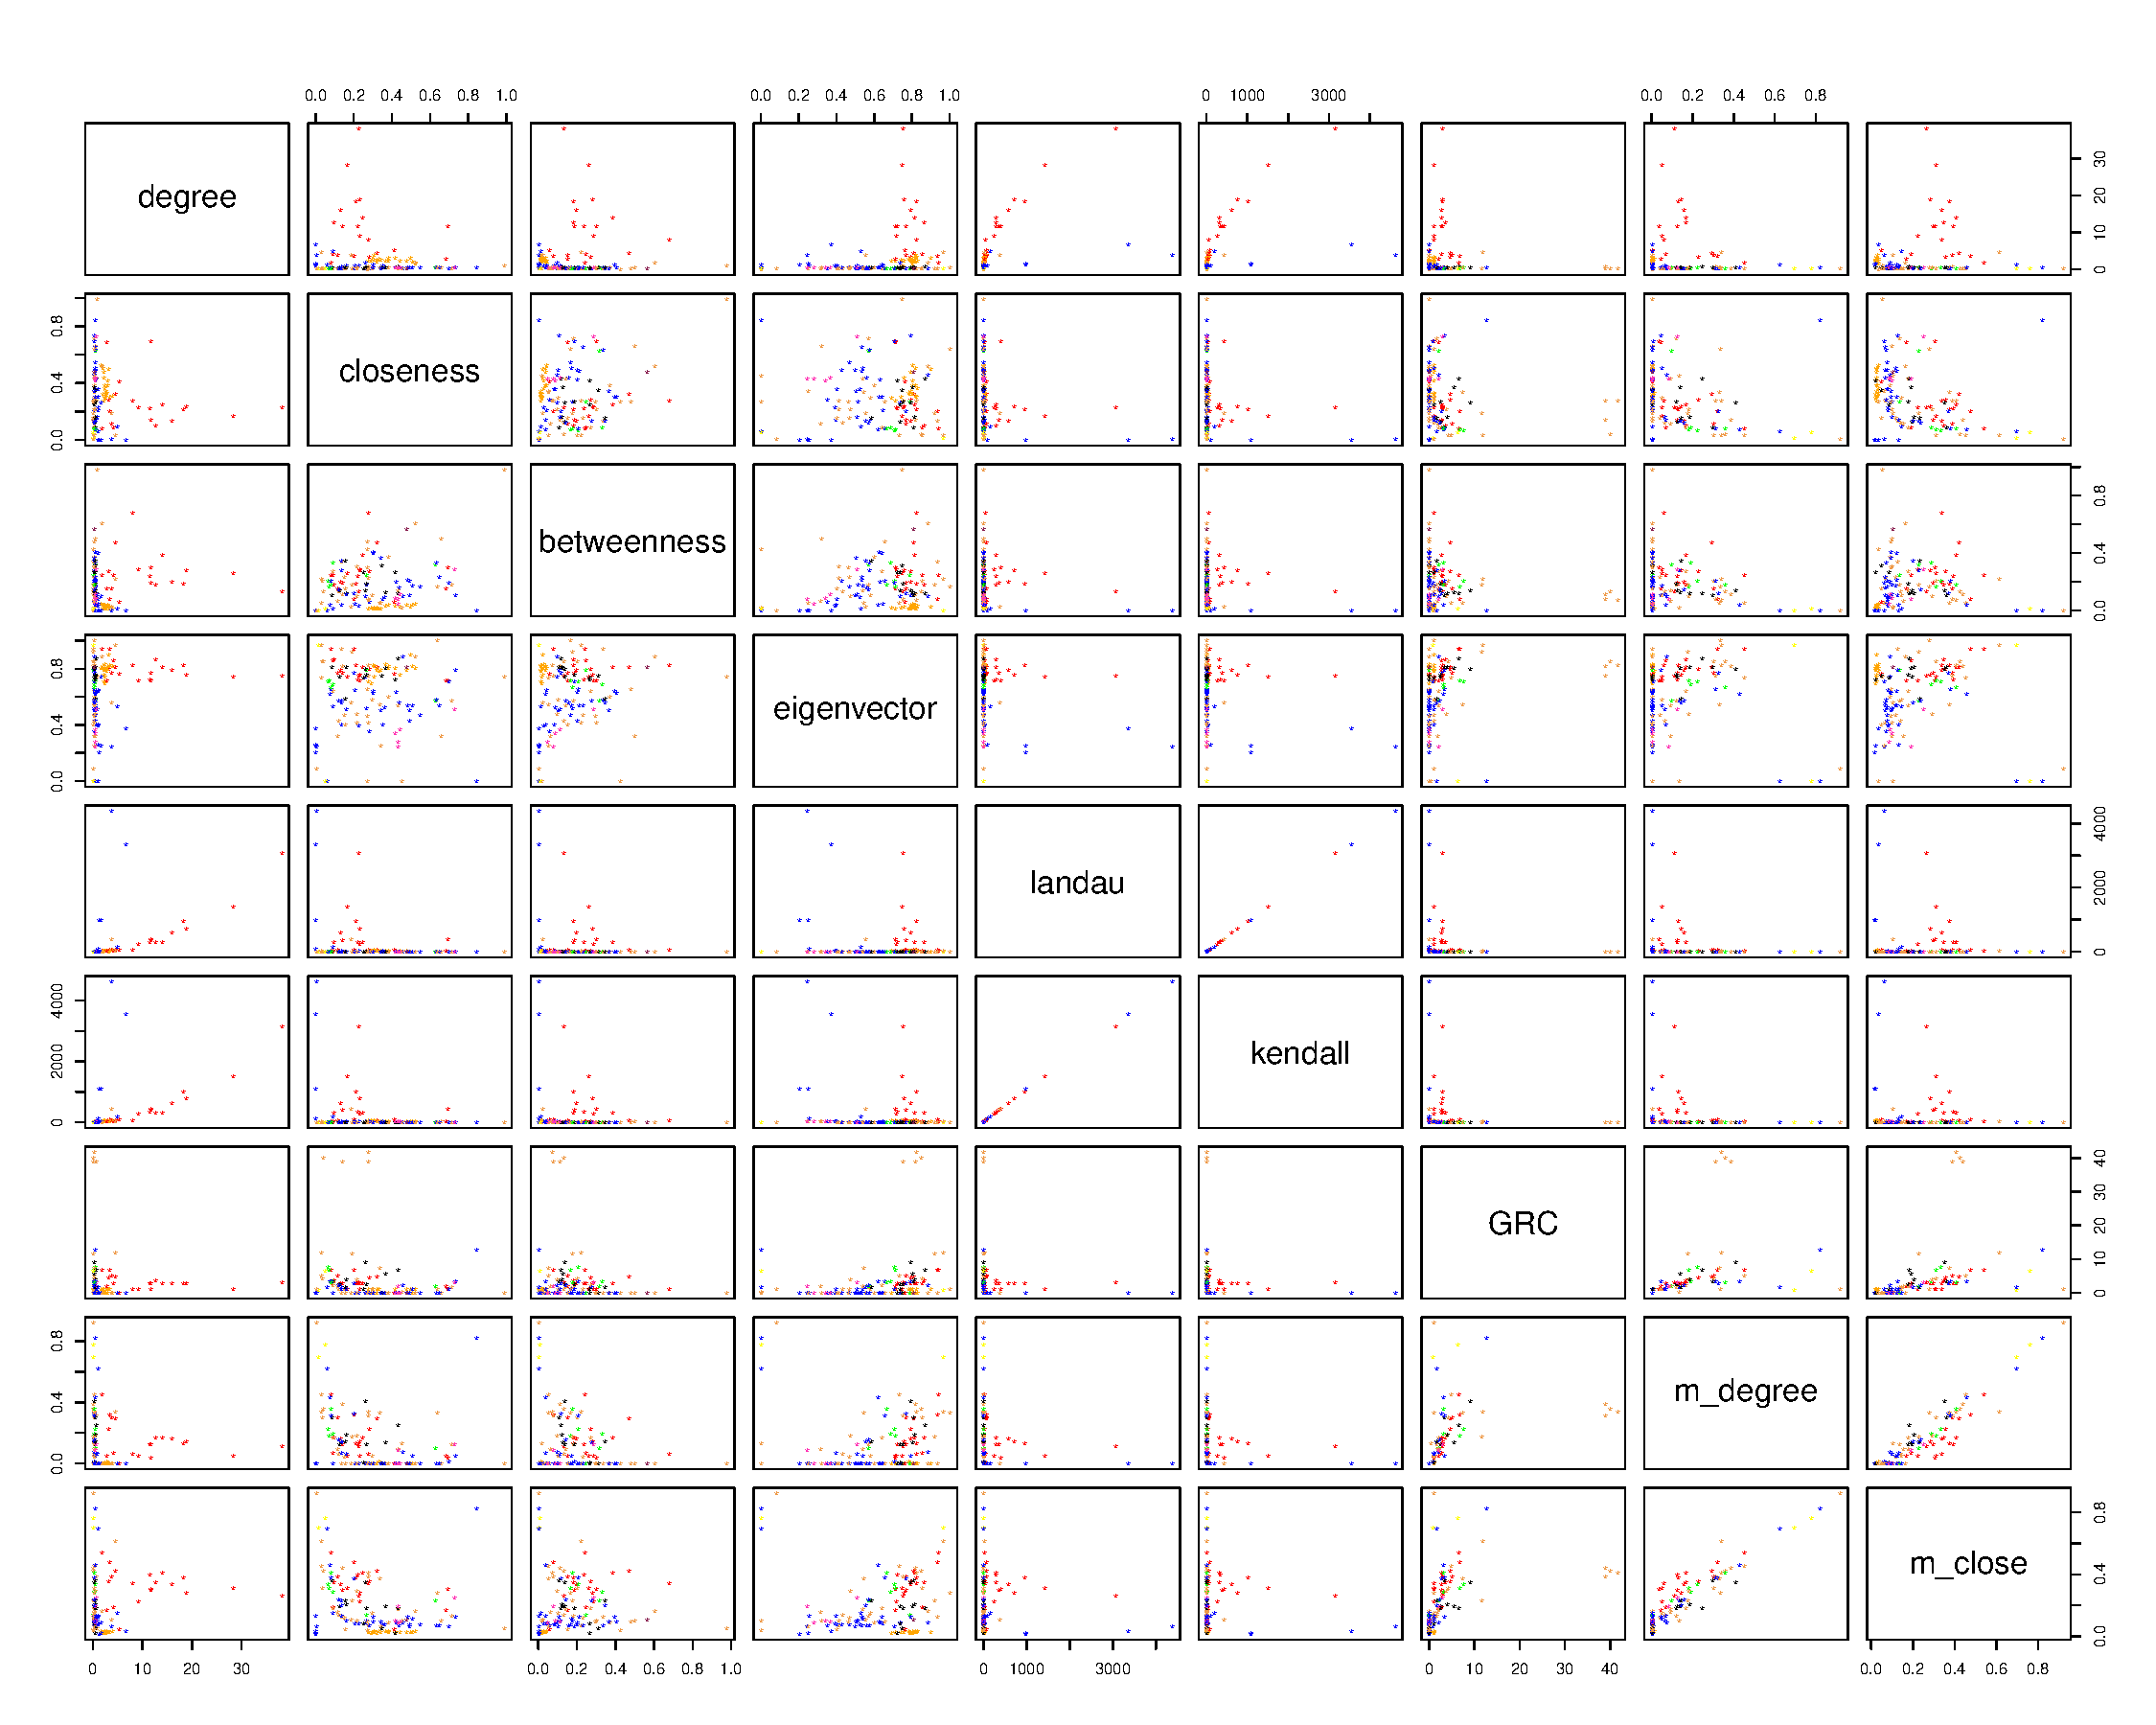
\includegraphics[width=12cm, height=8cm]{images/Global_Measure_Pairs_Plots.pdf}
	\end{changemargin}
\end{frame}

\begin{frame}\frametitle{Hiearchy in Networks -- PCA}
\begin{changemargin}{-2cm}{ -2cm}
		\centering
		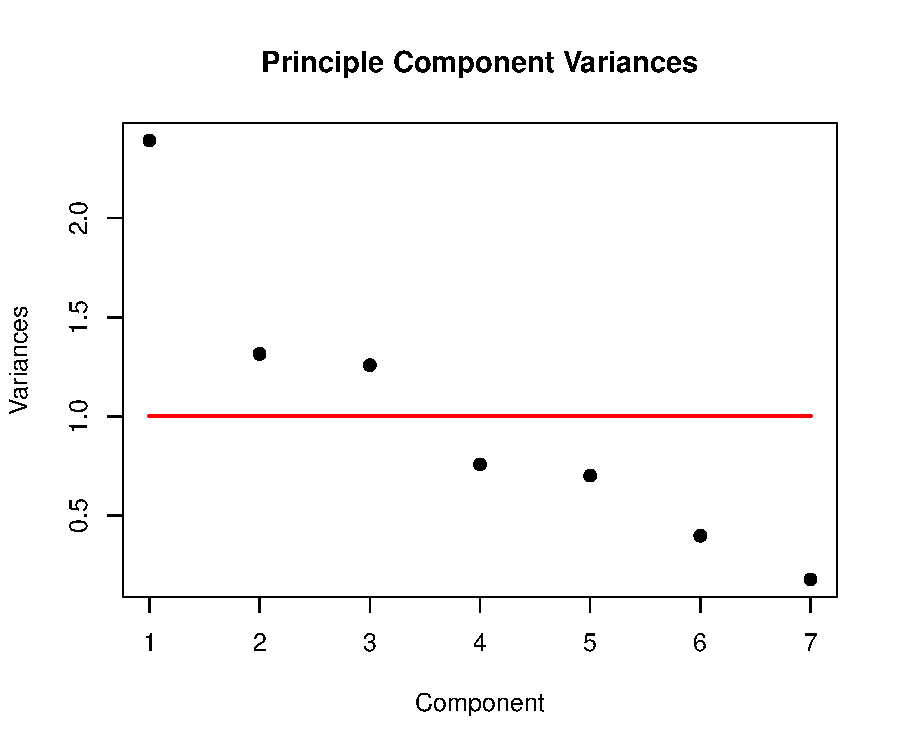
\includegraphics[scale = 0.6]{images/Observed_PCA_Component_Varinces.pdf}
%\begin{tikzpicture}
    %\node(a) at (10,4){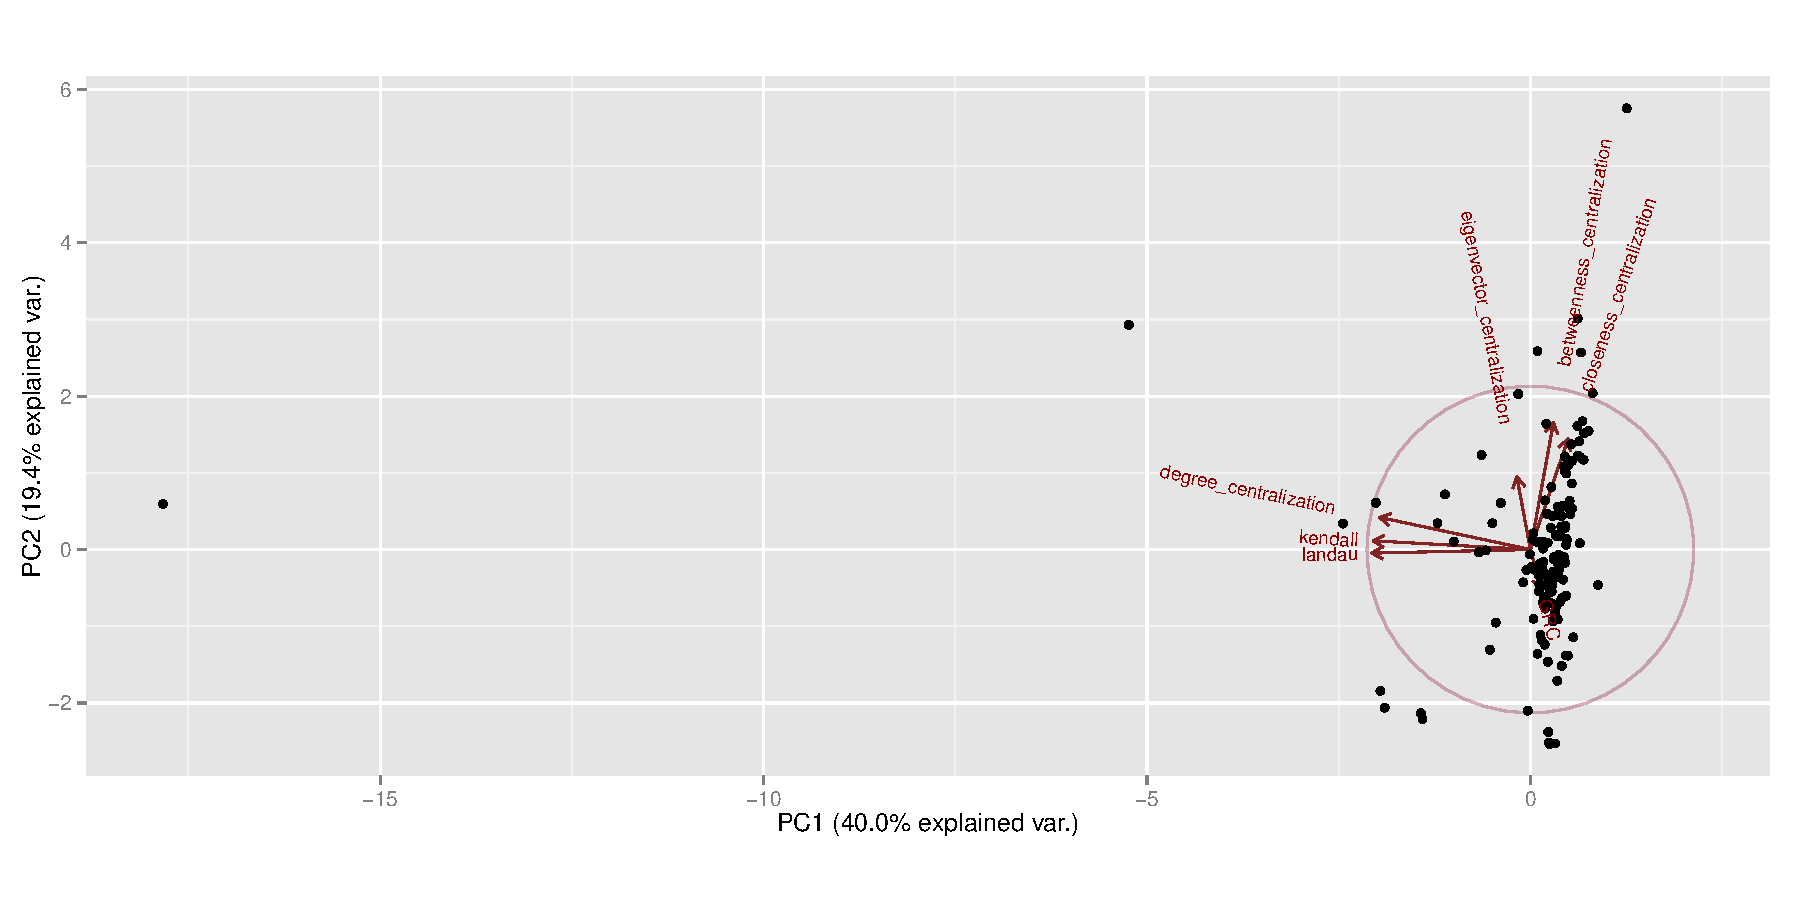
\includegraphics[width=12cm, height=8cm]{images/PCA_Plot}};
    %\pause
    %\node(b) at (5.5,6.5){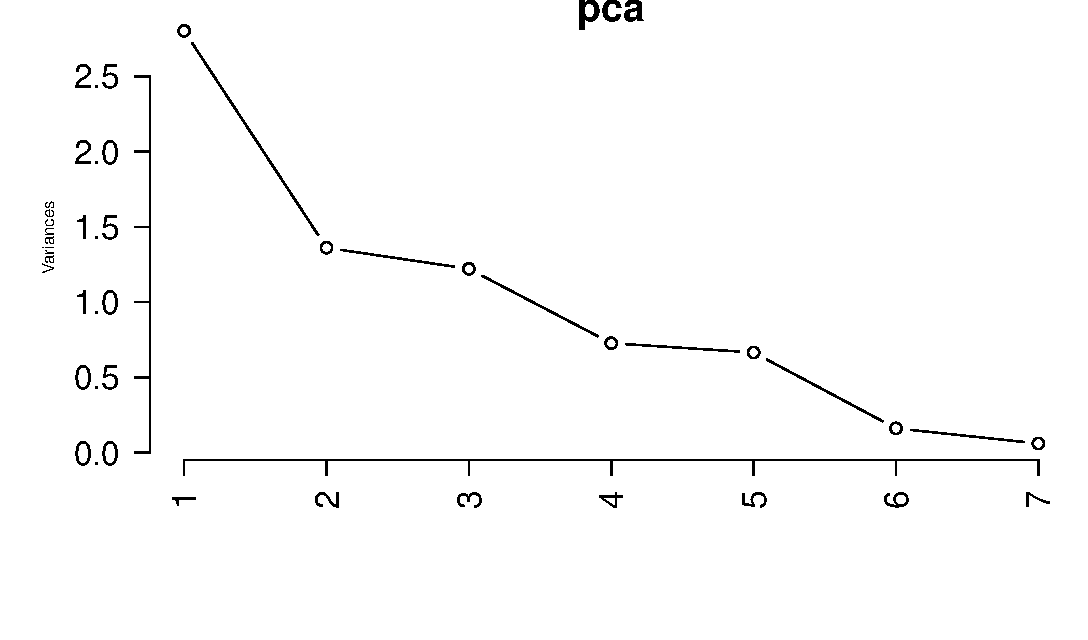
\includegraphics[width=4cm]{images/Eigenvalues}};
    %\draw[blue,->](11.1,5.6)--(8,0.5);
    %\draw[blue,->](12,5.5)--(4.5,4);
%  \end{tikzpicture}
\end{changemargin}
\end{frame}

\begin{frame}\frametitle{Hierarchy in Networks -- PCA}
	\begin{changemargin}{-2cm}{ -2cm}
		\centering
		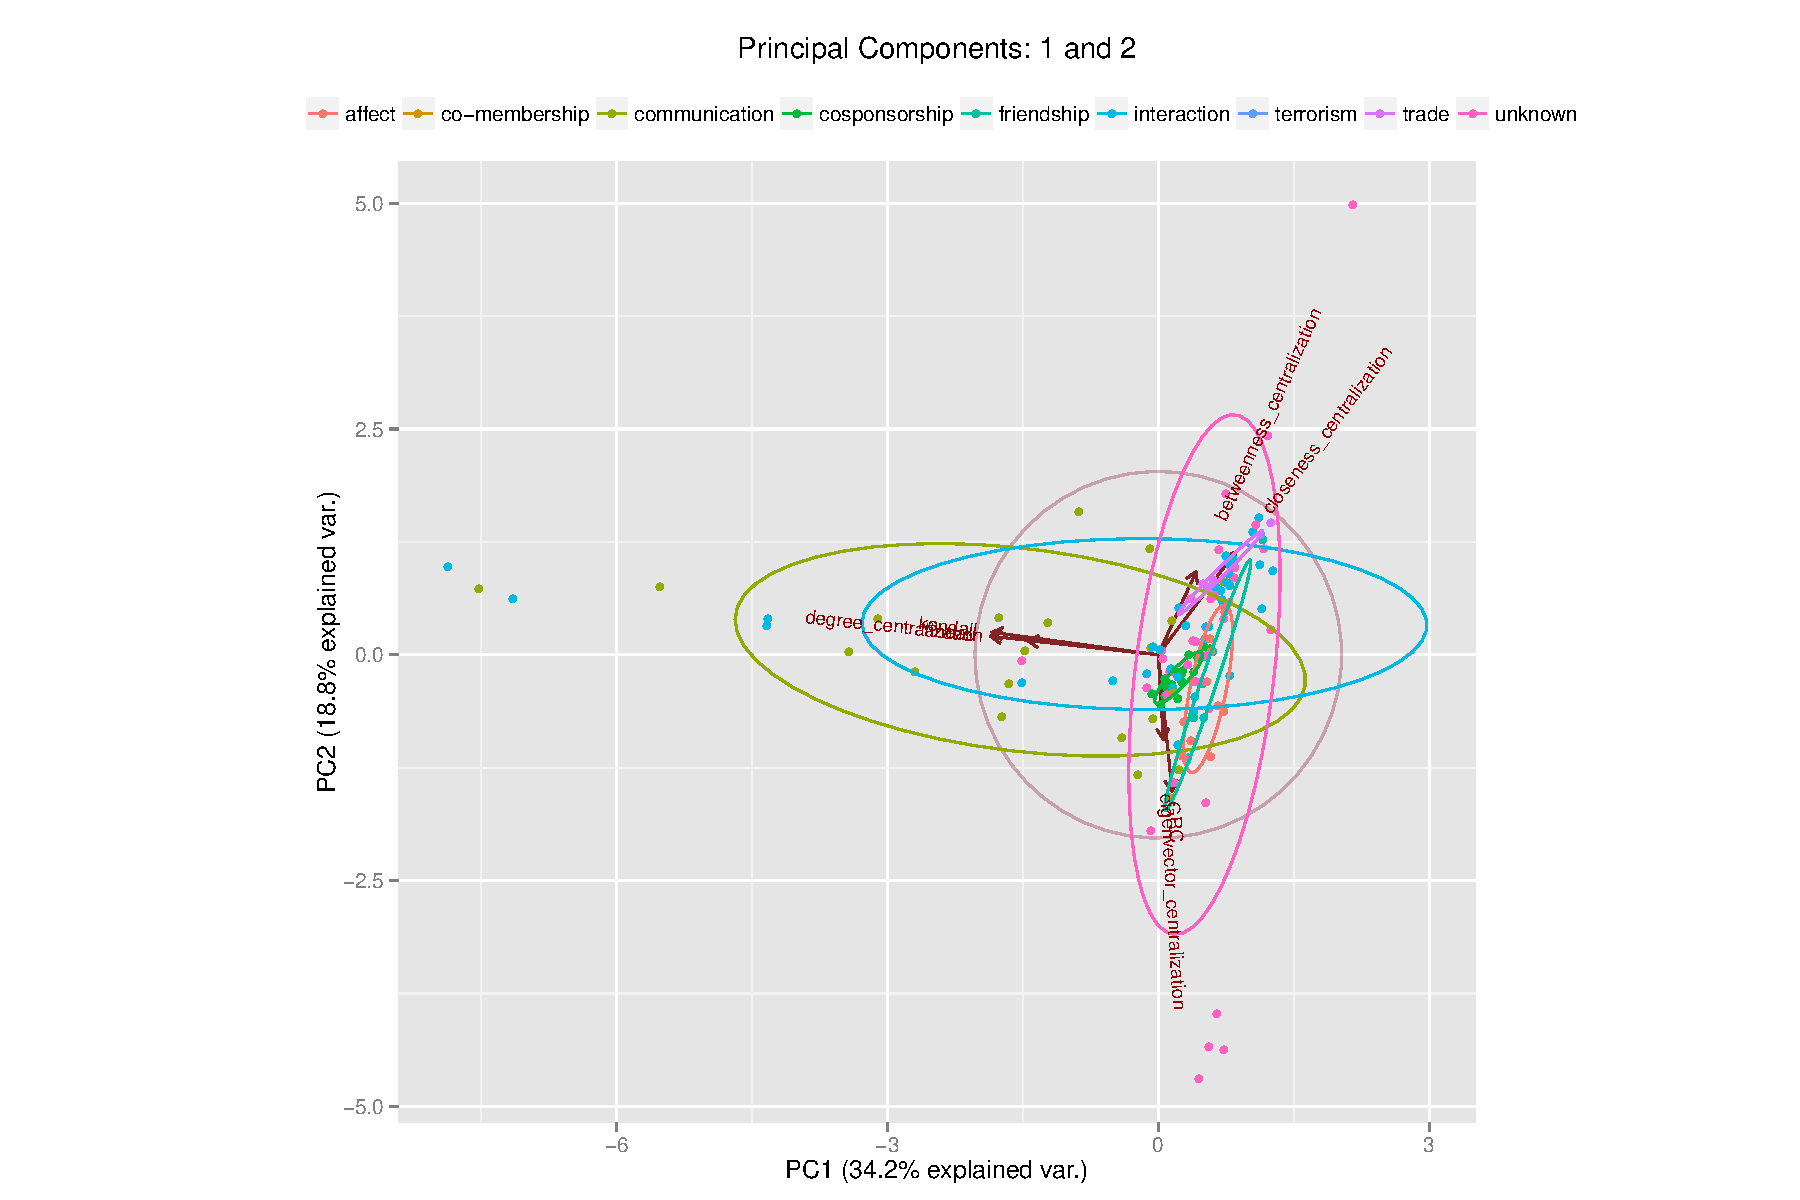
\includegraphics[width=12cm, height=8cm]{images/Observed_PCA_Components1_2.pdf}
	\end{changemargin}
\end{frame}

\begin{frame}\frametitle{Hierarchy in Networks -- PCA}
	\begin{changemargin}{-2cm}{ -2cm}
		\centering
		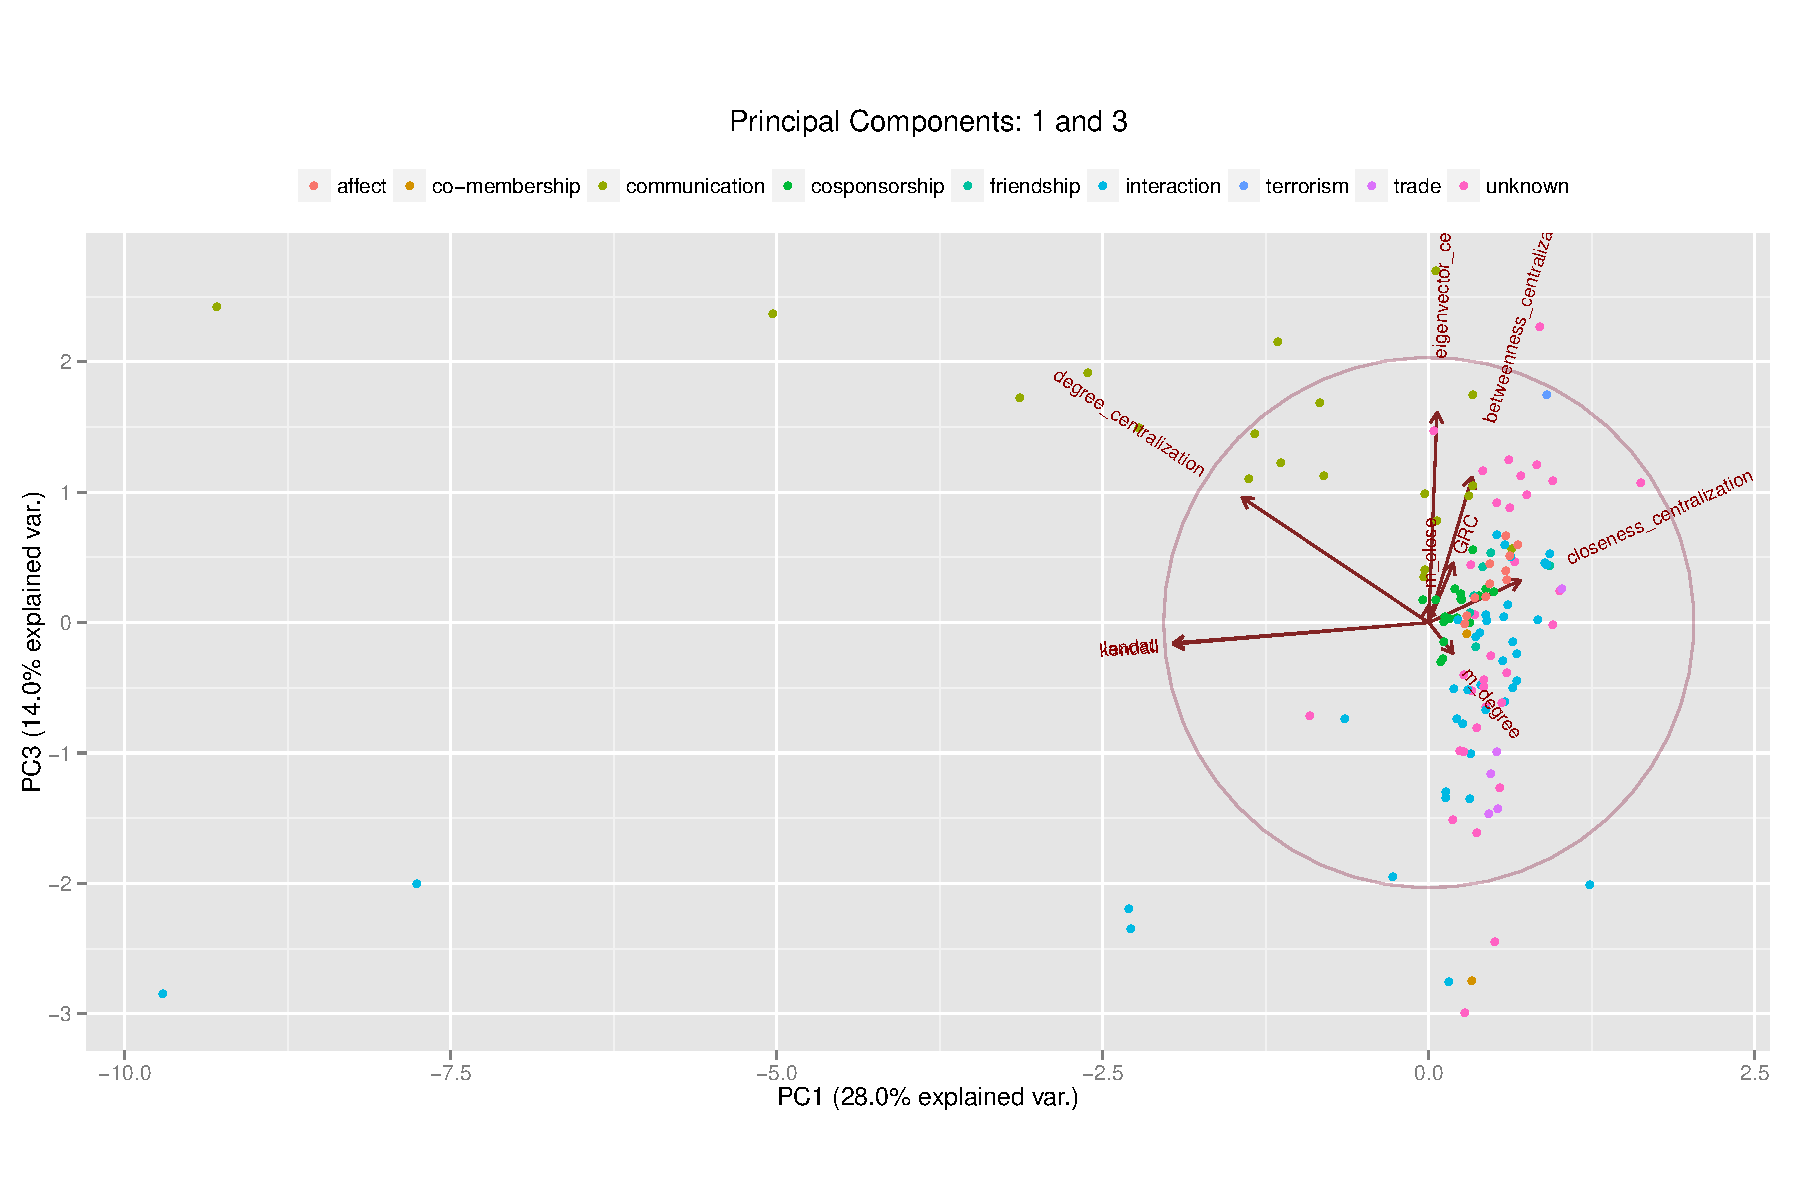
\includegraphics[width=12cm, height=8cm]{images/Observed_PCA_Components1_3.pdf}
	\end{changemargin}
\end{frame}

\begin{frame}\frametitle{Hierarchy in Networks -- PCA}
	\begin{changemargin}{-2cm}{ -2cm}
		\centering
		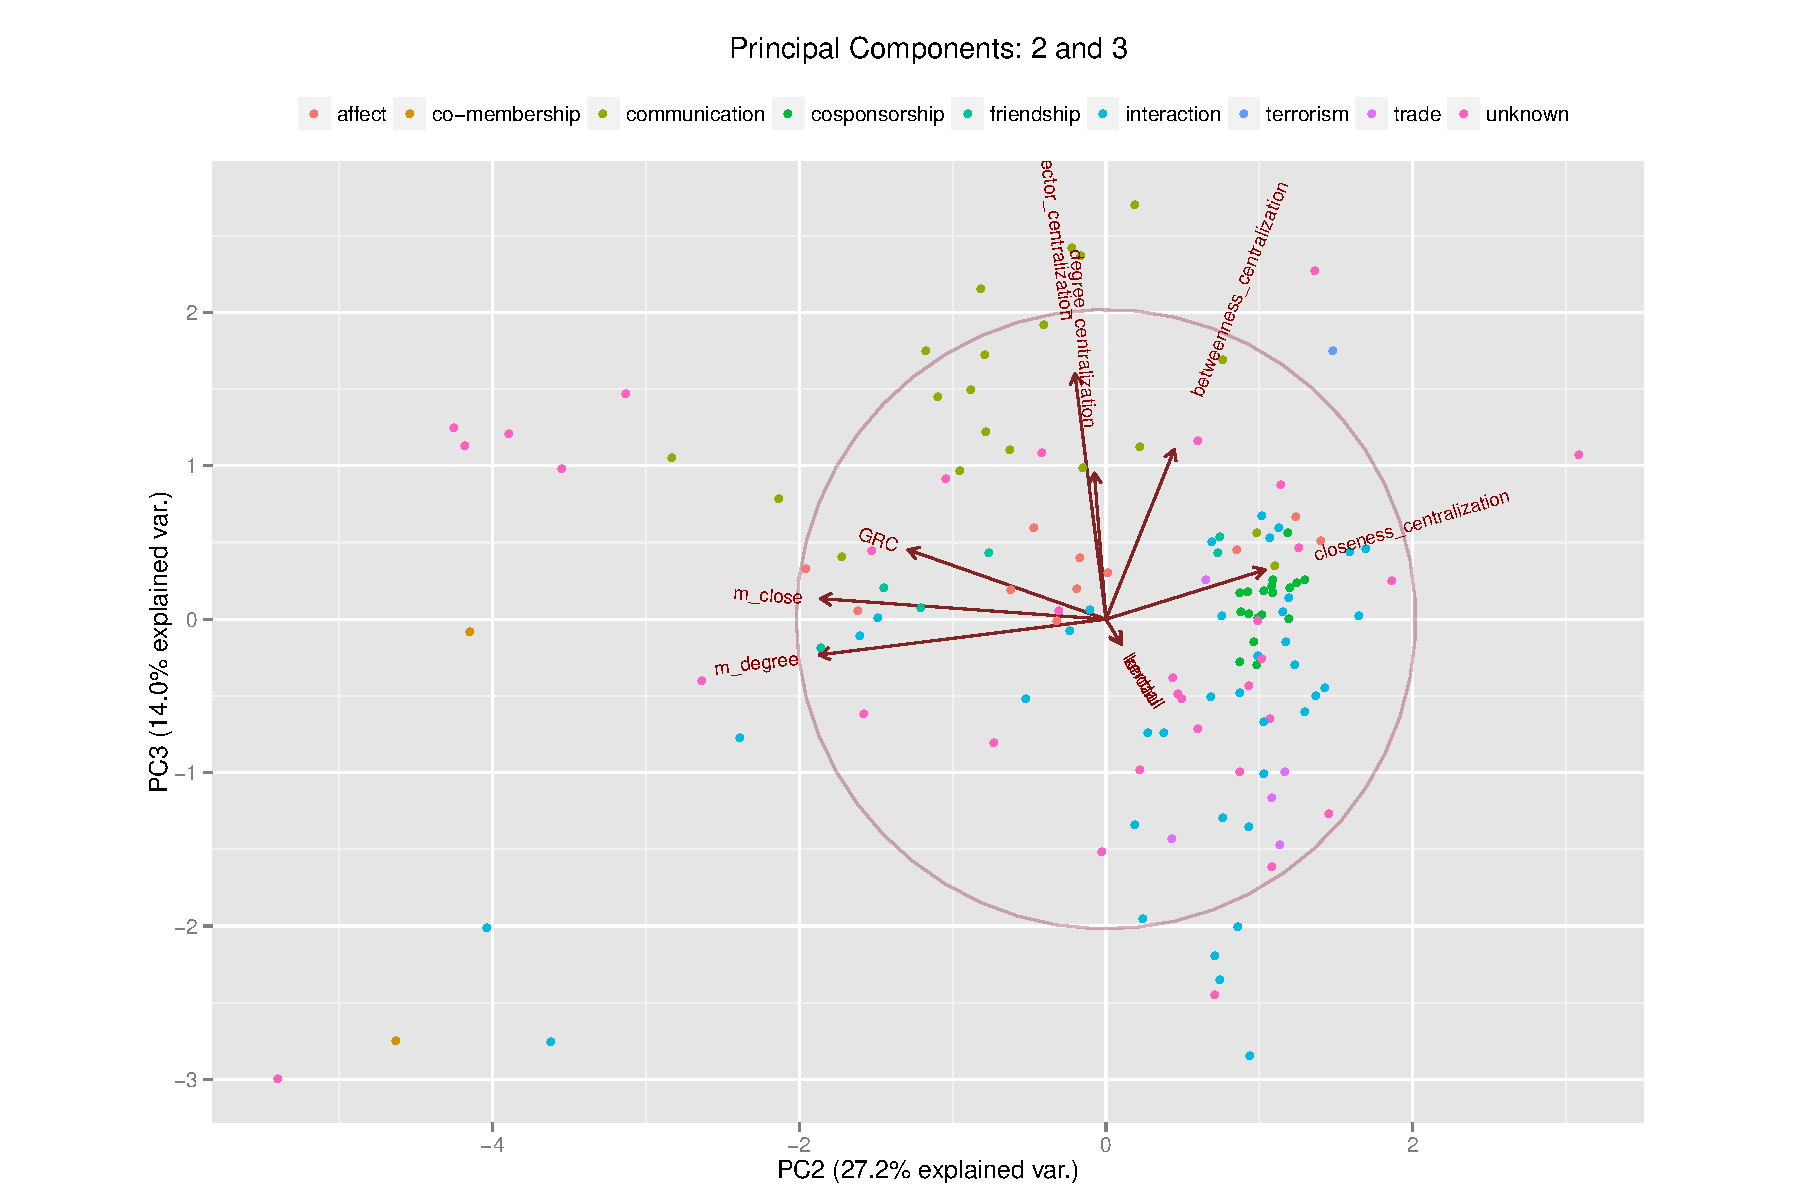
\includegraphics[width=12cm, height=8cm]{images/Observed_PCA_Components2_3.pdf}
	\end{changemargin}
\end{frame}

\begin{frame}\frametitle{Hierarchy in Networks--Results}
	\begin{itemize}
		\item Need first three principle components to explain the variation.
		\item Both trade and co-membership stay grouped and towards the center. 
		\item Both Landau and Kendall stay in same direction.
		\item From the first PCA plot (PC1~PC2), we notice that there are three clear groupings of measures.
		\item PC3 tries to separate the grouping of Betweenness from Landau and Kendall. 
	\end{itemize}
\end{frame}

\begin{frame}\frametitle{Hierarchy in Networks -- Local Measures}
	\begin{changemargin}{-2cm}{ -2cm}
		\centering
		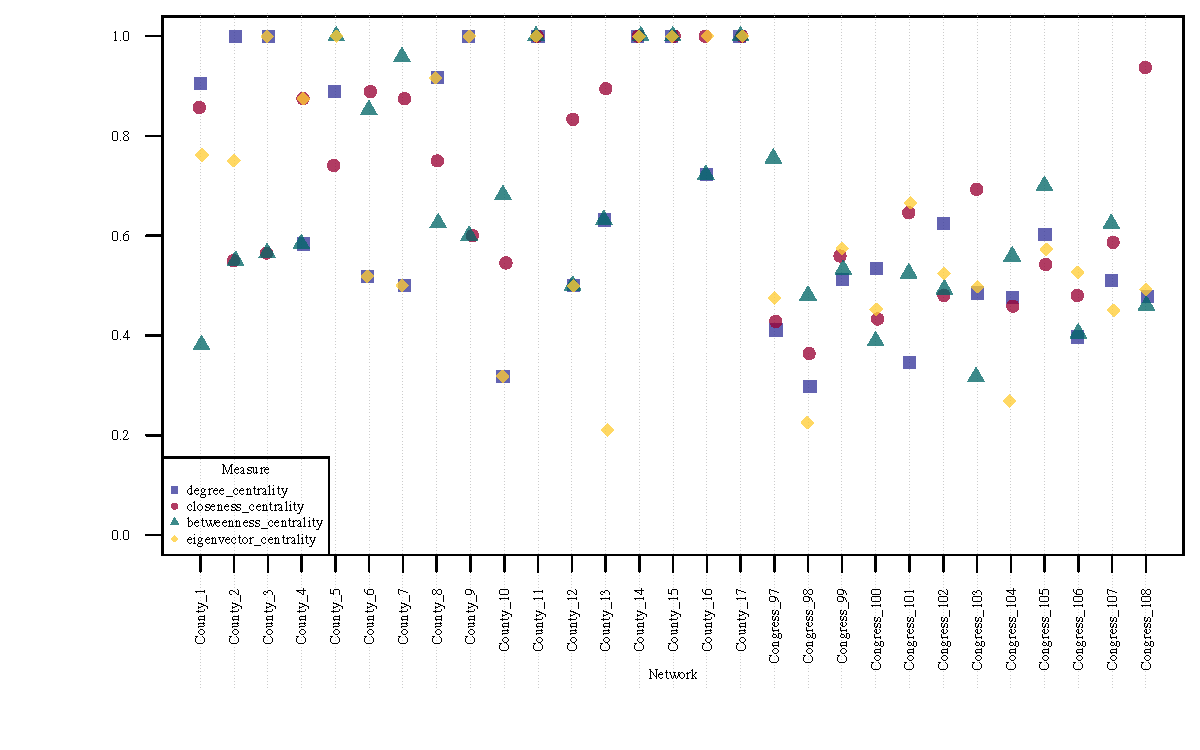
\includegraphics[width=12cm, height=8cm]{images/Measure_Scores.pdf}
	\end{changemargin}
\end{frame}
\end{document}
